% ---------------------------------------------------
% ----- Chapters of the template
% ----- for Bachelor-, Master thesis and class papers
% ---------------------------------------------------
%  Created by C. Müller-Birn on 2012-08-17, CC-BY-SA 3.0.
%  Freie Universität Berlin, Institute of Computer Science, Human Centered Computing. 
%
\chapter{Umsetzung}
\label{chap:implementation}
		
		Die im Rahmen dieser Masterarbeit entwickelte Software hat den Namen
		\textit{Simple Ontology Matcher} erhalten und besteht aus einem modularen Kern
		und ist über verschiedene Technologien ansprechbar. Aktuell sind die Module
		der Software als App für Django\footnote{\url{https://www.djangoproject.com/}} verfügbar, können
		aber auch direkt in Python Skripten benutzt werden.\\
		Der Kernteil besteht aus mehreren Modulen, um verschiedene Arten von
		Daten einlesen zu können, z. B.
		Formate wie OWL/XML, Query Languages wie SPARQL oder REST-Schnittstellen.
		Zusätzlich können unterschiedliche Arten und Implementierungen von Matchern
		verwendet werden. Um dies zu realisieren, gibt es eine Klasse, um Ontologien,
		deren Elemente und Eigenschaften abzubilden, namens \textit{ontology}.
		Die Elemente dieser Instanzen bestehen wiederum aus Instanzen der Klasse
		\textit{onto element}. Dort enthalten sind alle Informationen, die das Element
		beschreiben. Diese beiden Klassen dienen als Schnittstellen, um innerhalb der
		Software mit Ontologien und deren Elementen zu interagieren. Für diese beiden
		Teile können weitere Module implementiert werden, um zusätzliche
		Funktionalität zu erhalten, z. B. andere Datenquellen einzulesen.\\
		Die Wahl auf Python als verwendete Programmiersprache hatte zwei Gründe,
		Python ist weit verbreitet und bietet mit Django eine gute Möglichkeit, eine
		Web Applikation zu erstellen.
		
		\section{Architektur}
		Sowohl die Kernmodule als auch die einzelnen, konkreten Ausführungen dieser
		Module sind entlang eines Prozesses organisiert, wie in Abbildung \ref{fig2}
		gezeigt.
		\begin{figure}[h!]
		\centering
		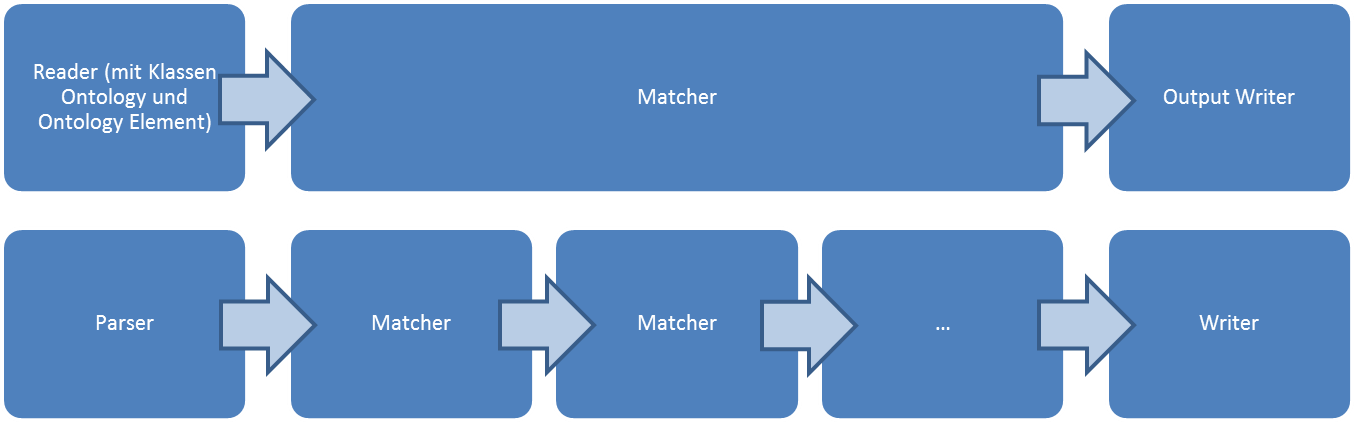
\includegraphics[width=1.0\textwidth]{pics/Module-overview.png}
		\caption{Prozessablauf der Module}
		\label{fig2}
		\end{figure}
		An erster Stelle stehen der oder die Parser, die die Ontologien einlesen und
		die Daten in Instanzen der Klasse \textit{ontology} einpflegen. Hierbei können
		auch Daten aus unterschiedlichen Quellen und beliebigen Formaten verwendet
		werden, sofern ein \textit{Reader} implementiert wurde. Im Rahmen dieser
		Masterarbeit wurden bereits einige implementiert, die einige gängige
		Möglichkeiten abdecken. Durch die Modularität können aber problemlos weitere
		hinzugefügt werden.\\
		Dann werden die Ontologien an verschiedene Matcher übergeben. Dabei werden
		die Ergebnisse von einem Matcher zum nächsten weitergegeben, so ist es zum
		einen möglich, diese Ergebnisse zu akkumulieren und zum
		anderen, weitergehende Analysen z. B. der Struktur oder Hierarchie vorzunehmen. Je nachdem, auf welche Eigenschaften
		eines Elements ein Matcher achtet, können sinnvolle Arten von Verbindungen
		festgelegt werden. Diese werden ebenfalls mit den einzelnen Matchings
		übergeben und später als Default Wert angezeigt. Die Gesamtergebnisse werden
		dann an einen \textit{Output Writer} übergeben, um sie dann weiter bearbeiten zu können.\\
		Sowohl die Reader als auch die Matcher Module haben Wrapper Module, die für
		die Interaktion zwischen den verschiedenen Modulen zuständig sind. Der
		Großteil der Programmlogik, der für die Verarbeitung des Input, also der
		Ontologien und der Matchings, benötigt wird, ist aber in den Readern und
		Matchern selbst enthalten. Die Wrapper Module enthalten nur ausreichend Logik,
		um die entsprechenden Module dynamisch einzubinden und den Input weiterzureichen.
		
		\cleardoublepage
		\pagebreak[4]
		
		\subsection{Anwendungsszenario 1: Django App}
		Um von nichttechnischen Experten leicht und ohne zusätzlichen Aufwand
		benutzbar zu sein, kann man die Module des Simple Ontology Matchers als App
		einer Django Installation verwenden. Die involvierten Module und der
		Pfad, der bei einem Matching Prozess durchlaufen wird, ist in Abbildung
		\ref{fig3} abgebildet. Über ein
		Skript\footnote{SimpleOntologyMatcher/OntologyMatcher/settings.py} von Django
		werden mögliche Ontologien und Matcher gesammelt.
		
		\begin{figure}[h!]
		\centering
		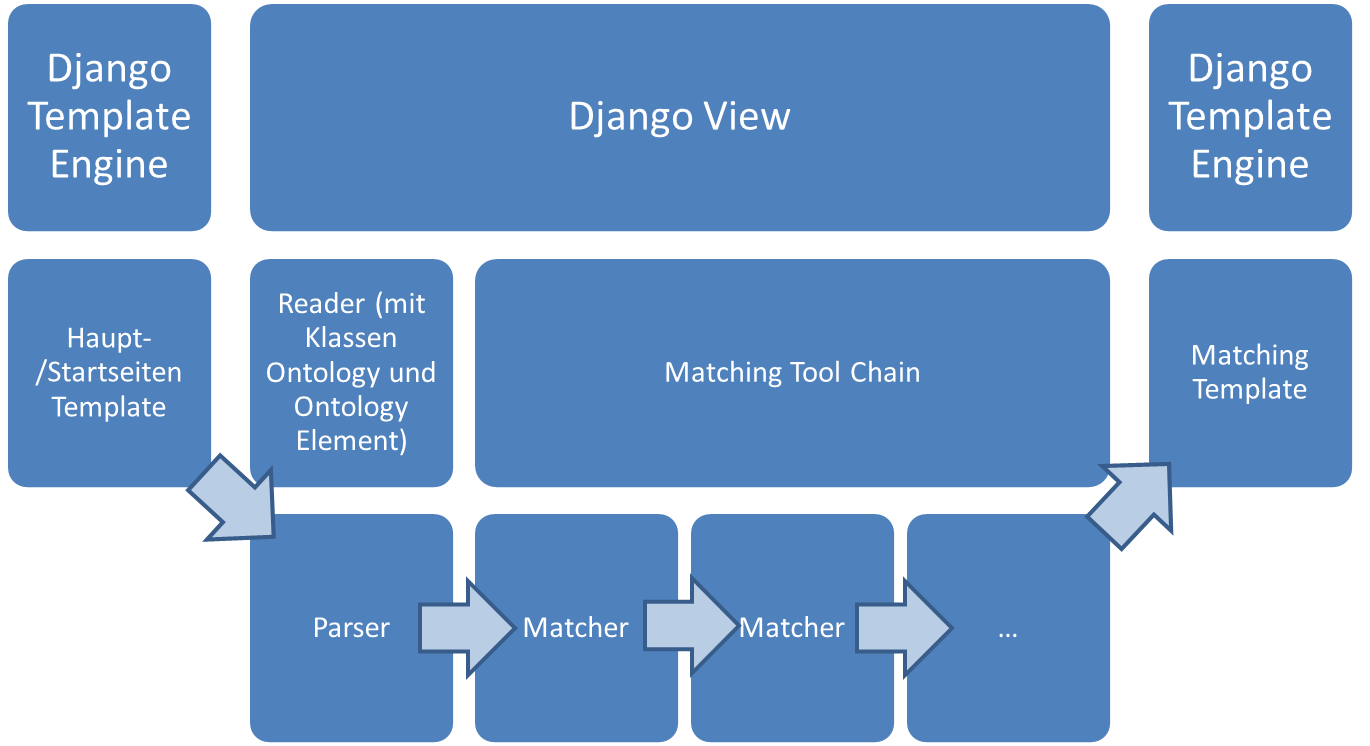
\includegraphics[width=1.0\textwidth]{pics/Module-overview1.png}
		\caption{Module Django App}
		\label{fig3}
		\end{figure}
		
		Beim Prozess können, wie erwähnt, verschiedene Quellen verwendet werden. Für
		Ontologien sind lokale und auf externen Servern gespeicherte Dateien und in
		Datenbanken eingepflegte Daten möglich. Bei Matchern werden nur lokal
		vorhandene Python Module berücksichtigt. Die gefundenen Ontologien und Matcher werden dann in
		ein HTML Template eingebettet, dass mit der \textit{Django Template Engine}
		erstellt wird. Dabei wird auch die Quelle gespeichert, also der Dateiname mit Pfad oder die URL.
		
		\pagebreak[4]
		
		Über die dann erstellte Seite können Ontologien, die
		analyisert werden sollen, ausgewählt werden und Matcher, mit denen dies durchgeführt wird.\\
		Das Design ist möglichst simpel gewählt, wie in \ref{fig4} gezeigt. Es gibt
		keine Menüs oder Einstellmöglichkeiten, sondern es können nur
		lokale oder externe Ontologien und Matcher ausgewählt
		werden. Die simple Oberfläche verbirgt auch die Komplexität, die im Backend
		und den Matching Algorithmen steckt, da sie für den nichttechnischen Experten
		nur bedingt von Interesse ist.\\
		Ontologien können dabei aus verschiedenen Quellen stammen. Aktuell
		sind lokal auf dem Server gespeicherte und externe Ontologien, wie
		die Terminologien vom GFBio Terminology
		Server\footnote{\url{http://terminologies.gfbio.org/}} als Quellen festgelegt.
		Durch die Auslassung von Konfigurationsmöglichkeiten wird die Bedienung
		vereinfacht, aber gleichzeitig die Komplexität verringert. Die GUI ist auf
		das Nötigste reduziert. Ein einfaches User Interface hilft auch bei der Akzeptanz, da der
		Einstieg ohne Vorkenntnisse auch für nichttechnische Experten erleichtert
		wird. Es ist keine Installation oder Konfiguration für den Anwender nötig,
		insbesondere wird außer einem Browser keine zusätzliche Software beim Anwender
		vorausgesetzt.
		
		\pagebreak[4]
		
		\subsection{Matching Prozessablauf}
		Auf den nächsten Seiten wird beispielhaft und mit Bildern der Matching Prozess
		mit dem Simple Ontology Matcher dargestellt.\\
		Nach dem Aufruf der URL erscheint die in Abbildung \ref{fig4} gezeigte
		Startseite und es kann direkt mit dem Matching Prozess begonnen werden.\\
		\begin{minipage}{\linewidth}
			\makebox[\linewidth]{
				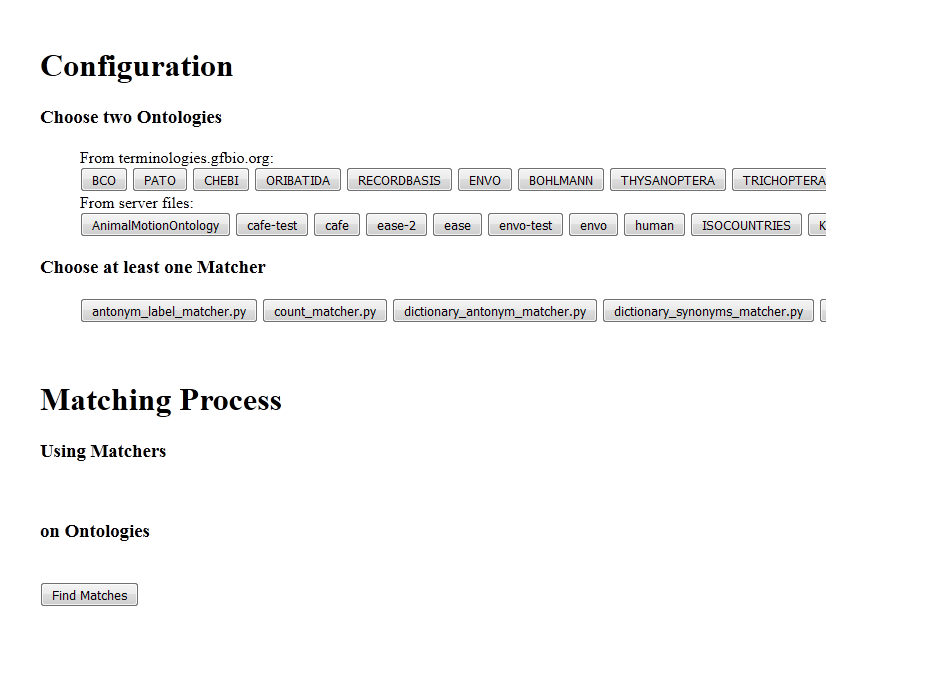
\includegraphics[keepaspectratio=true,width=0.8\textwidth]{pics/SimpleOntologyMatcher.png}}
			\captionof{figure}{Startseite Django App}\label{fig4}
		\end{minipage}
		
		Zuerst werden zwei Ontologien aus beliebigen Quellen und ein oder
		mehrere Matcher durch klicken auf die entsprechenden Buttons ausgewählt,
		die in Abbildung \ref{fig5} hervorgehoben wurden.\\
		\begin{minipage}{\linewidth}
			\makebox[\linewidth]{
				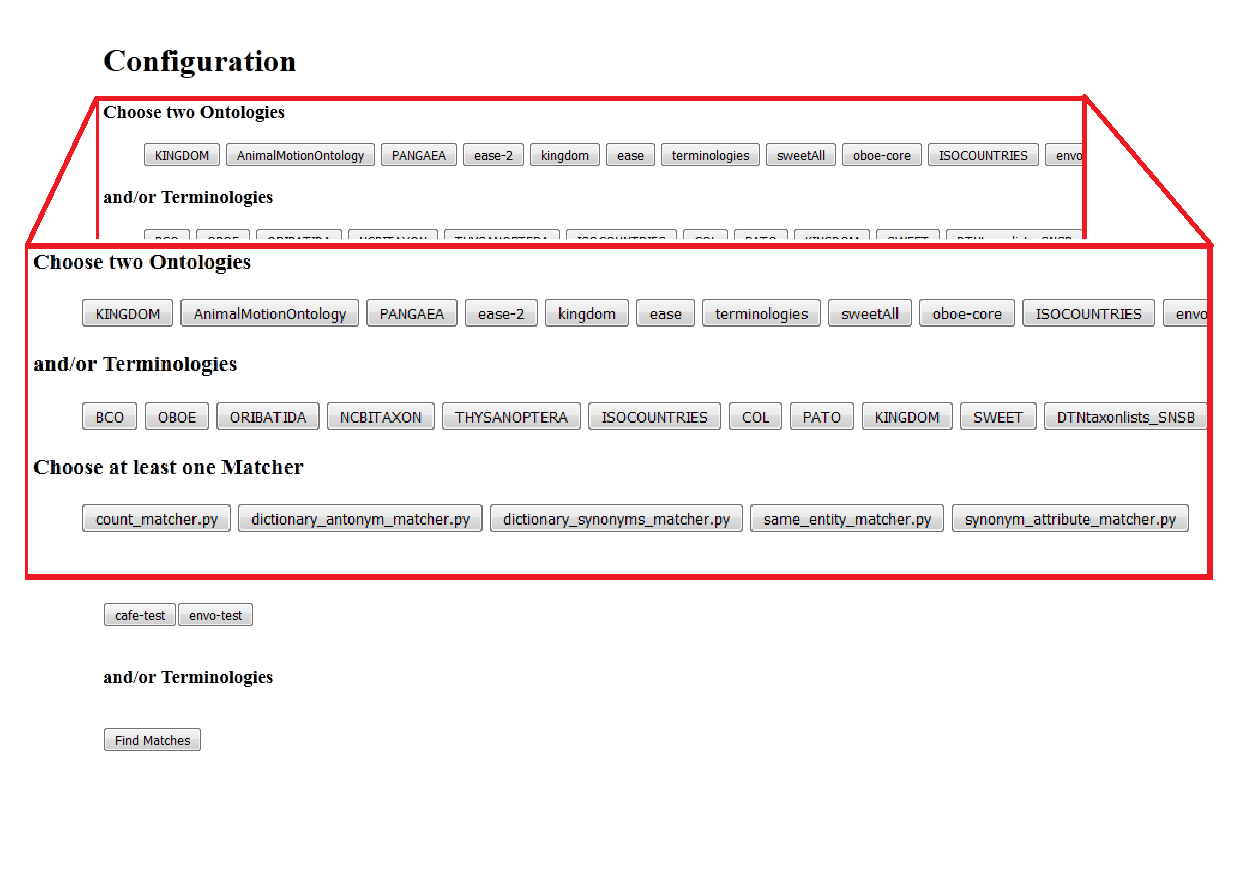
\includegraphics[keepaspectratio=true,width=0.8\textwidth]{pics/SimpleOntologyMatcher-Process.png}}
			\captionof{figure}{Matching Prozess Django App 1}\label{fig5}
		\end{minipage}
		
		\pagebreak[4]
		
		Die vom Benutzer ausgewählten Ontologien und Matcher werden
		unten angezeigt, wie Abbildung \ref{fig6} dargestellt.
		Dort können sie auch abgewählt werden, indem man auf die entsprechenden
		Buttons klickt.
		Die Matcher werden in der unten aufgeführten Reihenfolge ausgeführt. Das ist
		besonders bei den Matchern wichtig, die auf vorhergehende Ergebnisse zugreifen
		oder diese benötigen.\\
		\begin{minipage}{\linewidth}
			\makebox[\linewidth]{
				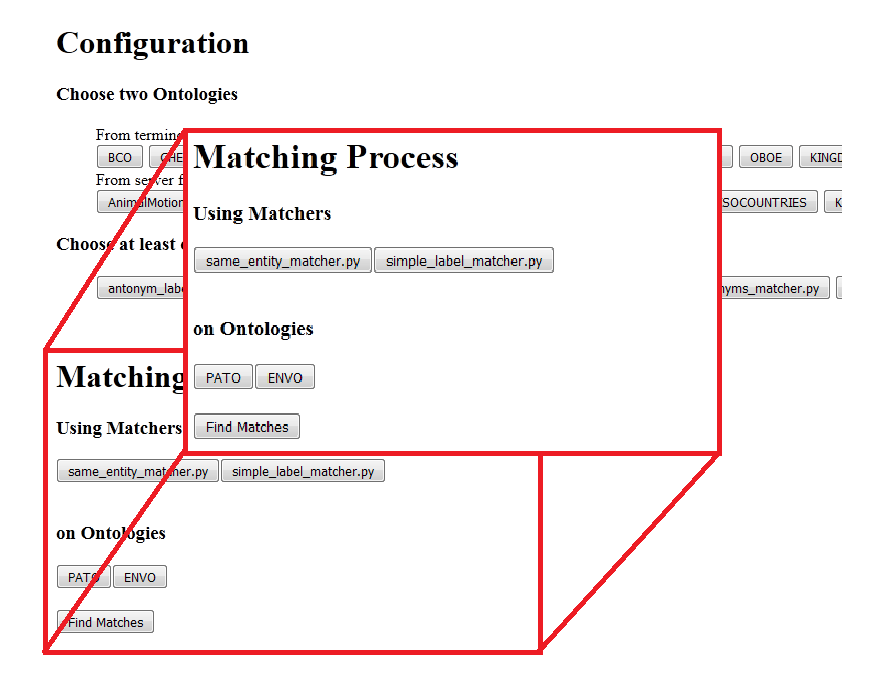
\includegraphics[keepaspectratio=true,width=0.8\textwidth]{pics/SimpleOntologyMatcher-Process1.png}}
			\captionof{figure}{Matching Prozess Django App 2}\label{fig6}  
		\end{minipage}
		\\
		Anschließend kann der Matching Prozess durch einen Klick auf \textit{Find
		Matches} gestartet werden, siehe Abbildung \ref{fig7}.\\
		\begin{minipage}{\linewidth}
			\makebox[\linewidth]{
				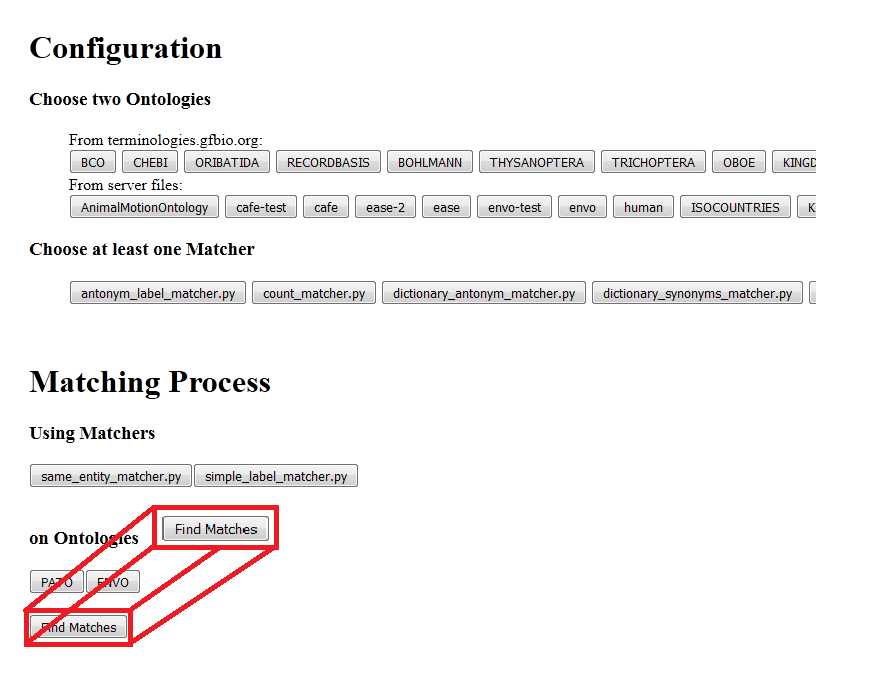
\includegraphics[keepaspectratio=true,width=1.0\textwidth]{pics/SimpleOntologyMatcher-Process2.png}}
			\captionof{figure}{Matching Prozess Django App 3}\label{fig7}  
		\end{minipage}
		\\
		Wenn der Matching Prozess abgeschlossen ist, wird eine Ergebnisseite
		angezeigt, wie in Abbildung \ref{fig8} dargestellt.\\
		\begin{minipage}{\linewidth}
			\makebox[\linewidth]{
				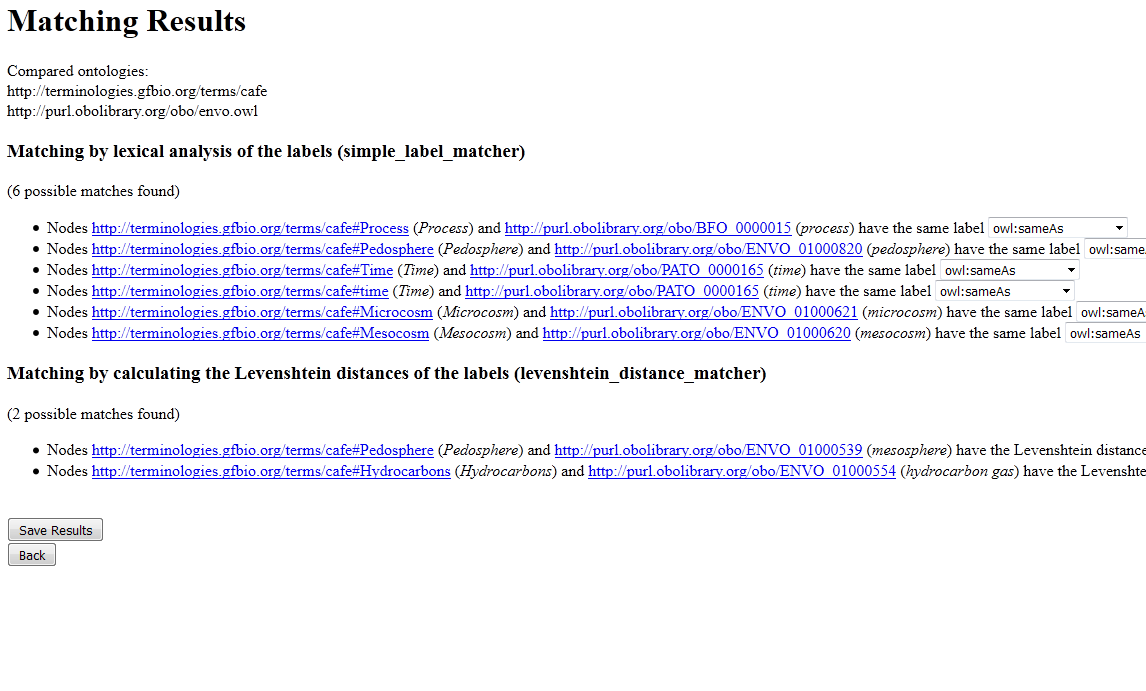
\includegraphics[keepaspectratio=true,width=1.0\textwidth]{pics/SimpleOntologyMatcher-Process3.png}}
			\captionof{figure}{Matching Prozess Django App 4}\label{fig8}  
		\end{minipage}
		
		Dort werden, wie in Abbildung \ref{fig9} hervorgehoben, oben die ausgewählten
		Ontologien angezeigt.\\
		\begin{minipage}{\linewidth}
			\makebox[\linewidth]{
				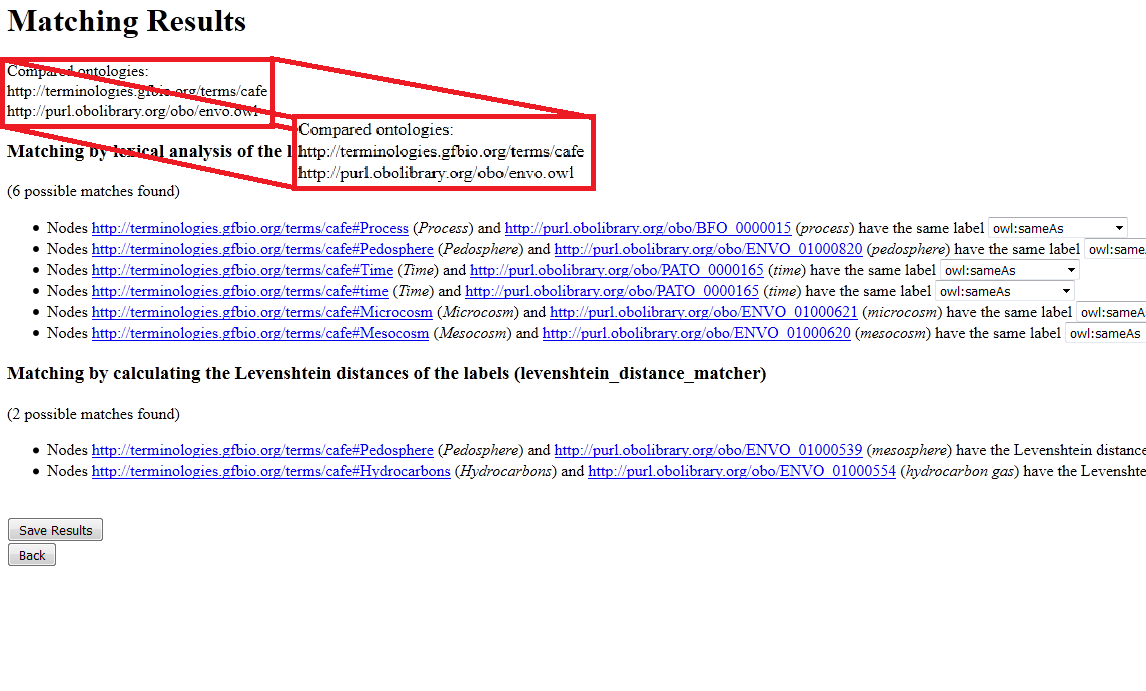
\includegraphics[keepaspectratio=true,width=1.0\textwidth]{pics/SimpleOntologyMatcher-Process4.png}}
			\captionof{figure}{Matching Prozess Django App 5}\label{fig9}  
		\end{minipage}
		
		\pagebreak[4]
		
		Die Matchings sind in verschiedene Kategorien unterteilt, für
		jeden Matcher eine, wie in Abbildung \ref{fig10} exemplarisch gezeigt.\\
		\begin{minipage}{\linewidth}
			\makebox[\linewidth]{
				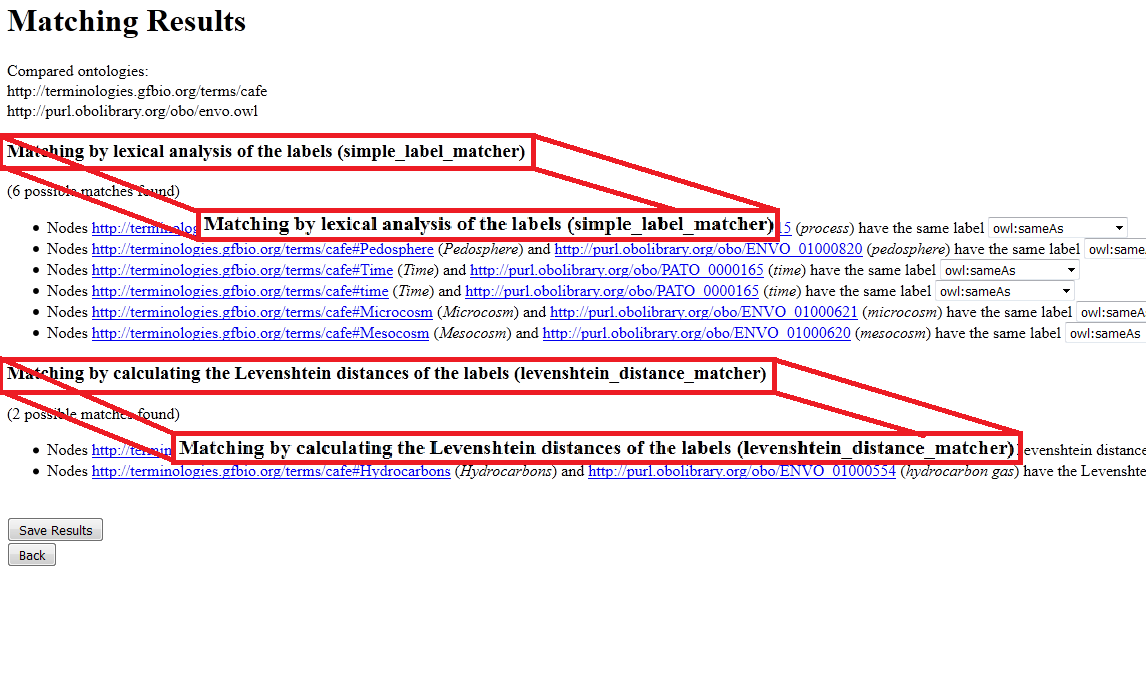
\includegraphics[keepaspectratio=true,width=1.0\textwidth]{pics/SimpleOntologyMatcher-Process5.png}}
			\captionof{figure}{Matching Prozess Django App 6}\label{fig10}  
		\end{minipage}
		\\
		In den Kategorien sind die gefundenen Matchings aufgeführt, wie Abbildung
		\ref{fig11} hervorhebt.\\
		\begin{minipage}{\linewidth}
			\makebox[\linewidth]{
				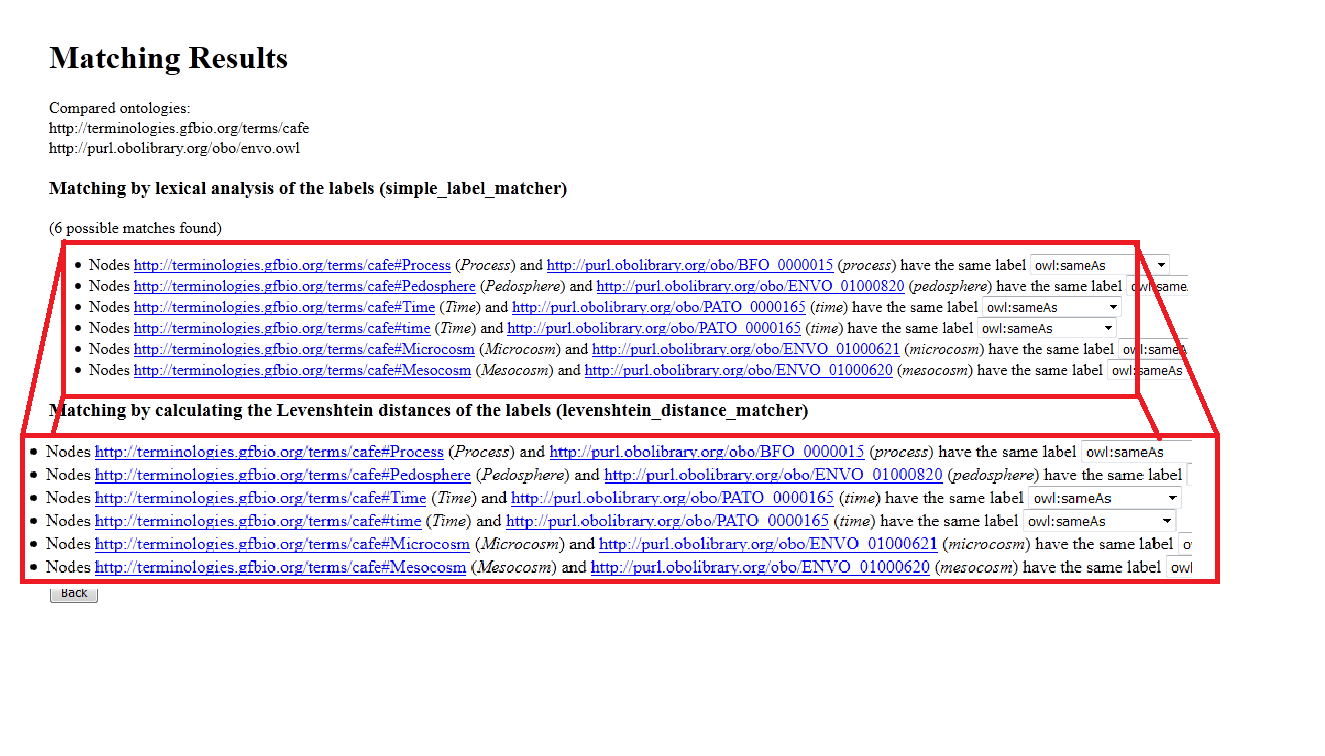
\includegraphics[keepaspectratio=true,width=1.0\textwidth]{pics/SimpleOntologyMatcher-Process6.png}}
			\captionof{figure}{Matching Prozess Django App 7}\label{fig11}
		\end{minipage}
		
		\pagebreak[4]
		
		Die einzelnen Zeilen enthalten ein Matching Paar, wie in Abbildung \ref{fig12}
		hervorgehoben. Angezeigt werden die URIs, die Labels, sofern vorhanden, eine
		kurze Begründung, warum dieser Matcher dieses Matching vorschlägt.\\
		\begin{minipage}{\linewidth}
			\makebox[\linewidth]{
				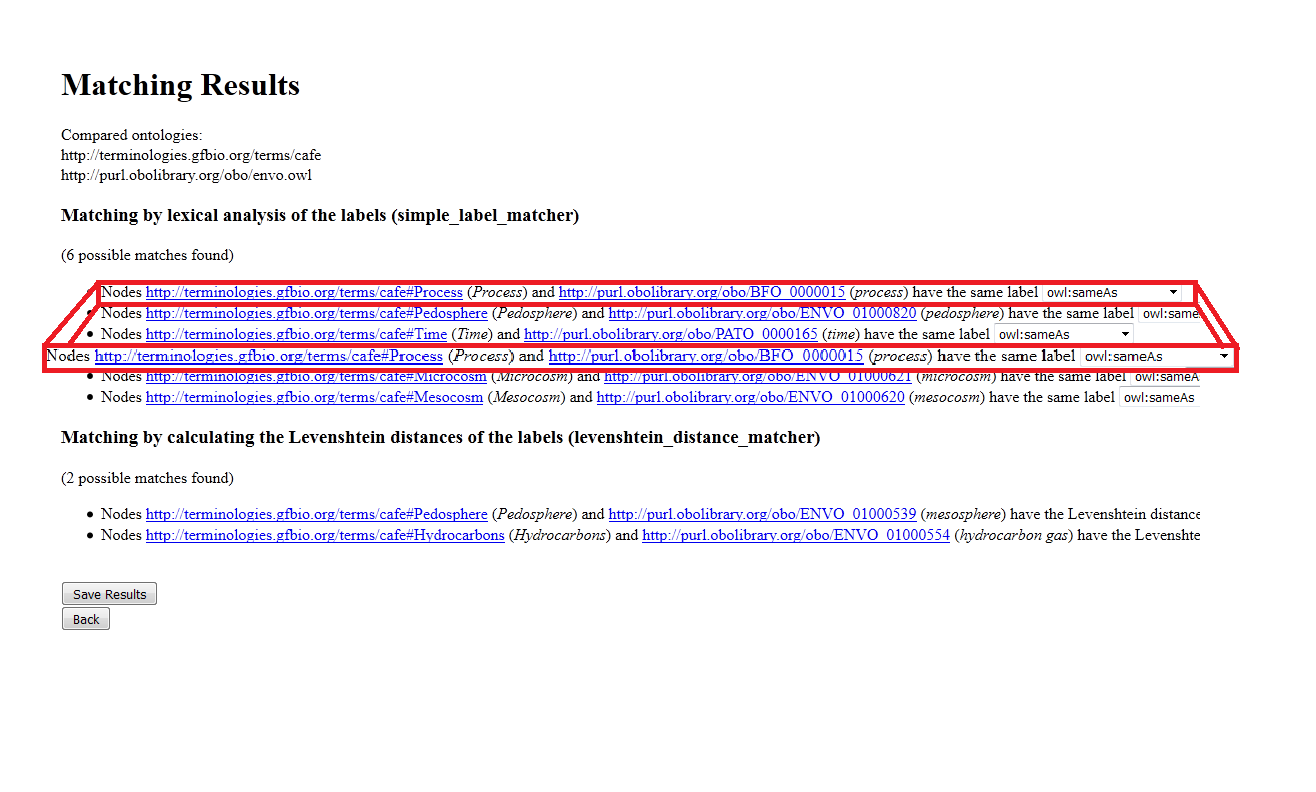
\includegraphics[keepaspectratio=true,width=1.0\textwidth]{pics/SimpleOntologyMatcher-Process7.png}}
			\captionof{figure}{Matching Prozess Django App 8}\label{fig12}  
		\end{minipage}
		\\
		Zusätzlich gibt es ein Dropdown Menü, aus dem ausgewählt werden kann, wie und
		ob eine Verbindung zwischen diesen zwei Elementen besteht, siehe Abbildung \ref{fig13}. Da es für
		einige Matcher sinnvolle Verbindungstypen gibt, sind diese bereits als Default
		Wert angewählt. Das wird vom jeweiligen Matcher bestimmt. Zur Auswahl für
		Verbindungen stehen eine Reihe von im \textit{Web Ontology Language} (OWL)
		Standard definierten.
		Axiomen.\footnote{\url{https://www.w3.org/TR/owl-ref/}}\\
		\begin{minipage}{\linewidth}
			\makebox[\linewidth]{
				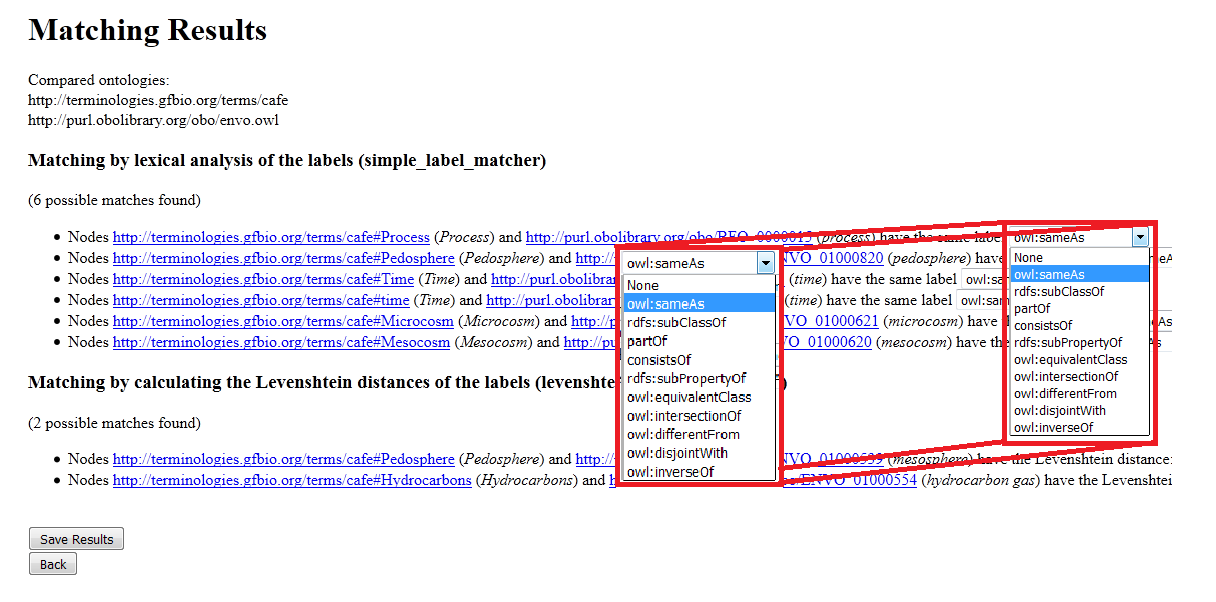
\includegraphics[keepaspectratio=true,width=1.0\textwidth]{pics/SimpleOntologyMatcher-Process9.png}}
			\captionof{figure}{Matching Prozess Django App 9}\label{fig13}  
		\end{minipage}
		
		\pagebreak[4]
		
		Durch einen Klick auf \textit{Save Results}, siehe Abbildung \ref{fig14}, kann
		man die bestätigten Verbindungen und ihre Elemente in RDF XML exportieren. Matchings für die keine
		Verbindung ausgewählt wurde, werden nicht gespeichert.\\
		\begin{minipage}{\linewidth}
			\makebox[\linewidth]{
				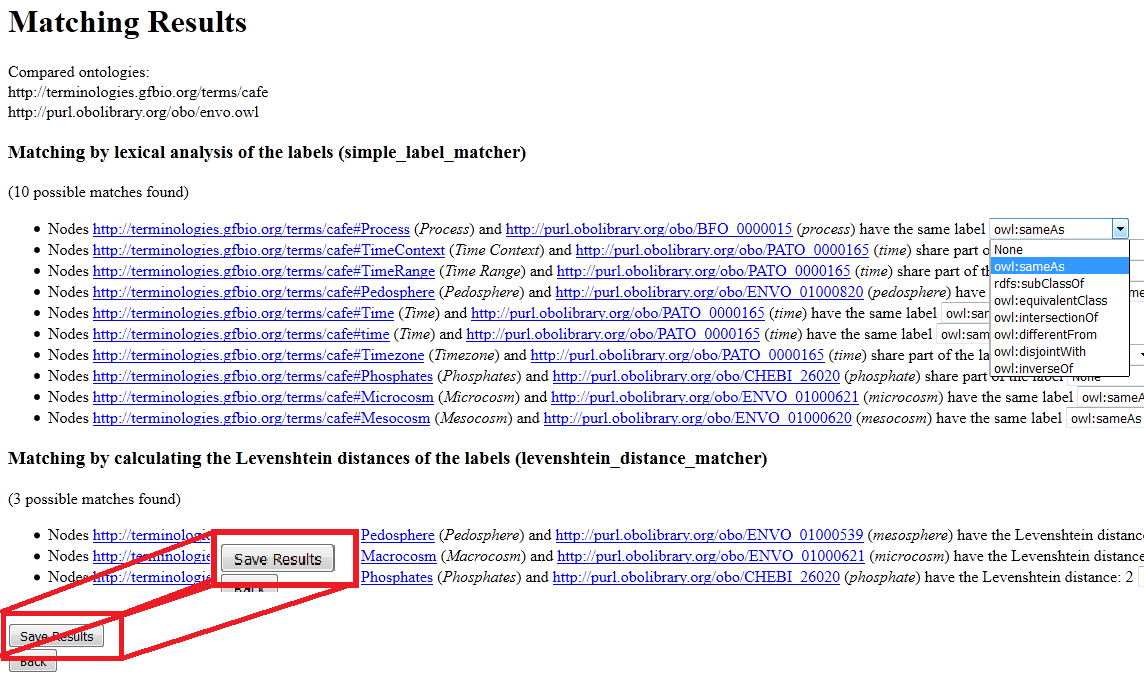
\includegraphics[keepaspectratio=true,width=1.0\textwidth]{pics/SimpleOntologyMatcher-Process10.png}}
			\captionof{figure}{Matching Prozess Django App 10}\label{fig14}  
		\end{minipage}
		\\
		In Abbildung \ref{fig15} ist exemplarisch der XML Code für ein Matching
		aufgeführt.\\
		\begin{minipage}{\linewidth}
			\makebox[\linewidth]{
				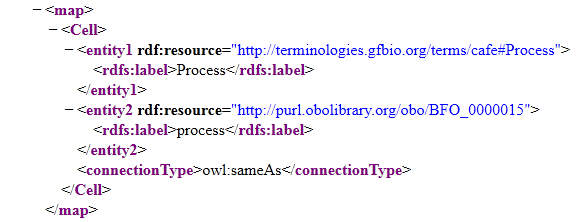
\includegraphics[keepaspectratio=true,width=1.0\textwidth]{pics/SimpleOntologyMatcher-Process11.png}}
			\captionof{figure}{Matching Prozess Django App 11}\label{fig15}  
		\end{minipage}
		
		\pagebreak[4]
		
		Intern werden die ausgewählten Ontologien mit entsprechenden
		\textit{Readern} geparst. Die Reader werden ermittelt, indem überprüft wird,
		ob es sich bei der gespeicherten Quelle um eine URL oder eine
		existierende und lesbare Datei handelt. Dies wird über das \textit{View} von
		Django durchgeführt und dann an das \textit{Reader} Modul weitergeleitet. Dieses
		bindet die passenden Module ein, startet das Parsen und liefert die Ergebnisse
		in Form einer Instanz der Klasse \textit{ontology} zurück. Die Ergebnisse
		aller Reader werden in einer Liste gesammelt.\\
		Mit den übergebenen Matchern wird eine \textit{Matching Tool Chain} im
		gleichnamigen Modul erstellt, welche die Matcher in der vom
		Benutzer ausgewählten Reihenfolge ausführt. Die Ergebnisse jedes Matching
		Vorgangs werden von einem Matcher an den nächsten in Form des Python Datentyps \textit{Dictionary}
		weitergegeben. Durch das weiterleiten der Ergebnisse zwischen den Matchern
		ist es möglich, auf vorherige Ergebnisse zuzugreifen, um z. B. die Struktur von
		Elementen innerhalb der Ontologien zu analysieren,
		siehe auch Kapitel \ref{StrukturellesMapping} Strukturelles Mapping.
		Die Ergebnisse eines Matchers werden dann zum Ergebnis Dictionary
		hinzugefügt.\\
		Wenn alle Matcher durchlaufen wurden, wird das letztendliche Ergebnis in einem
		anderen Template der Django Template Engine verarbeitet und angezeigt,
		wie in Abbildung \ref{fig7} exemplarisch dargestellt.
		
		\subsection{Anwendungsszenario 2: Python Skript}
		Neben der Möglichkeit den Simple Ontology Matcher als Django App und damit als
		Web service zu verwenden, können die einzelnen Module auch wie üblich als
		normale Python Module importiert und aufgerufen werden. Dabei ist es möglich, die Module der
		Zwischenschicht\footnote{matcher.py und reader.py} zu verwenden oder
		auszulassen, da diese nur das dynamische Einbinden übernehmen. Dieses
		Szenario erlaubt es technischen Experten, Module des Simple Ontology Matchers
		als Basis zu benutzen und den Vorgang des Ontology Matchings zu
		automatisieren und unabhängig von der GUI zu arbeiten.
		
		\section{Implementierte Reader}
		Um Ontologien aus verschiedenen Quellen nutzen zu können, wurden einige Reader
		implementiert, um die Ontologien zu parsen und die Inhalte der Ontologien in
		Instanzen der Klassen \textit{onto\_elem} aus dem Modul \textit{onto\_element}
		und \textit{ontology} aus dem gleichnamigen Modul zu überführen. Da alle
		Reader Instanzen dieser Klassen nutzen, können die Ontologien unabhängig von
		ihrem Ursprung auf die gleiche Weise verwendet werden.
		
		\subsection{RDF XML Parser}
		Mit diesem Reader werden lokal vorliegende XML Dateien geparst, in denen
		Ontologien im RDF Format enthalten sind.
		
		\subsection{OWL RDF XML Parser}
		Dieser Matcher unterscheidet sich in seinem Aufbau und Ablauf nur geringfügig
		vom RDF XML Parser. Es werden andere Elemente bzw. Tags erkannt, um die
		Ontologie einzulesen.
		
		\subsection{OWL RDF XML Web Parser}
		Damit auch externe Ressourcen für Ontologien verwendbar sind, wurde der OWL
		RDF XML Parser modifiziert, um Dateien aus Web Ressourcen anstatt lokale
		Dateien zu parsen.
		
		\subsection{GFBio Terminology Server Parser}
		Um Ontologien, die auf dem GFBio Terminology Server vorgehalten werden zu
		verwenden, wurde ein Reader implementiert, der erst alle Elemente der
		übergebenen Ontologie und dann die Attribute der einzelnen Elemente abfragt.
		
		\subsection{GFBio JSON Parser}
		Die Ontologien des GFBio Terminology Servers können auch im JSON Format
		heruntergeladen werden. Damit diese auch genutzt werden können, wurde
		dieser Reader implementiert. 
		
		\section{Implementierte Matcher}
		\label{ImplementierteMatcher}
		Im Rahmen dieser Masterarbeit wurden verschiedene Matching Algorithmen
		implementiert. Das Ziel der verschiedenen Matcher ist nicht nur Beziehungen,
		die Gleichheit oder Ähnlichkeit ausdrücken, zu finden, sondern möglichst
		verschiedene Arten von Verknüpfungen.
		
		\subsection{Same Entity Matcher}
		Der einfachste Matcher überprüft die URI der Elemente, um festzustellen, ob es
		in den übergebenen Ontologien gleiche Elemente gibt. Dies wird über eine
		einfache Abfrage auf Gleichheit der gesicherten URIs getan.
		\begin{lstlisting}
		for i in onto_elements:
			for j in onto1_elements:
				if re.match(i.name, j.name, re.IGNORECASE):
		\end{lstlisting}
		
		\subsection{Simple Label Matcher}
		\label{simpleOntologyMatcher}
		Bei diesem Matcher werden die Labels der Elemente auf Ähnlichkeiten
		untersucht.
		Zuerst werden die Labels auf exakte Gleichheit überprüft.
		\begin{lstlisting}
		match_result = re.match("^" + item.get_text().replace("_", " ") + "$", item1.get_text().replace("_", " "), re.IGNORECASE) if not already_matched and match_result and not re.match(i.name, j.name, re.IGNORECASE):
		\end{lstlisting}
		Anschließend wird nach Übereinstimmungen in den Labels gesucht.
		\begin{lstlisting}
		elif not exact_match and not already_matched and len(item.get_text()) > 3 and len(item1.get_text()) > 3 and not re.match(i.name, j.name, re.IGNORECASE):
            #check the first of the two labels
            if re.match("^" + item.get_text().replace("_", " ") + "\s", item1.get_text().replace("_", " "), re.IGNORECASE):
                connections["matches"].append([i.name, item.get_text(), j.name, item1.get_text(), " share part of the label\n", "dcterms:hasPart"])
                already_matched = True
            elif re.search("\s" + item.get_text().replace("_", " ") + "$", item1.get_text().replace("_", " "), re.IGNORECASE):
                connections["matches"].append([i.name, item.get_text(), j.name, item1.get_text(), " share part of the label\n", "rdfs:subClassOf"])
                already_matched = True
            elif re.match("^" + item1.get_text().replace("_", " ") + "\s", item.get_text().replace("_", " "), re.IGNORECASE):
                connections["matches"].append([i.name, item.get_text(), j.name, item1.get_text(), " share part of the label\n", "dcterms:partOf"])
                already_matched = True
            elif re.search("\s" + item1.get_text().replace("_", " ") + "$", item.get_text().replace("_", " "), re.IGNORECASE):
                connections["matches"].append([i.name, item.get_text(), j.name, item1.get_text(), " share part of the label\n", "rdfs:subClassOf"])
                already_matched = True
		\end{lstlisting}
		Die reguläre Ausdrucküberprüfung wird in beide Richtungen durchgeführt, da in
		den Python \textit{re.match} und textit{re.search} Funktionen der im ersten
		Argument übergebene Ausdruck im zweiten gesucht wird. In beiden Fällen darf
		der gesuchte Ausdruck aber nicht schon vorher als Match markiert worden sein,
		die gleiche URI besitzen oder kürzer als vier Zeichen sein.\\
		In früheren Tests, wo es die Einschränkung der Länge der Labels noch nicht
		gab, waren in der Ergebnismenge viele false positives. Zusätzlich wurde in
		früheren Versionen dieses Matchers einfach nach Vorkommen der Label Wörter in
		dem anderen Label geprüft. Dies führte ebenfalls zu vielen false positives.
		Dies wurde dann dahingehend geändert, dass der vollständige Ausdruck entweder
		am Anfang gefolgt von einem Leerzeichen stehen muss oder am Ende des Labels mit
		einem Leerzeichen direkt davor.
		
		\subsection{Levenshtein Distance Matcher}
		Dieser Matcher berechnet die Levenshtein Distanz bzw. den Editierabstand
		zwischen den Labels zweier Elemente. Also wie viele Änderungen der Buchstaben
		man an einem Label durchführen muss, um das andere Label zu erhalten.\\
		Zuerst wird geprüft, ob beide Label aus mehr als drei Buchstaben bestehen.
		Dann wird der Abstand zwischen beiden berechnet. Damit ein
		Elementenpaar als mögliches Matching anerkannt wird, muss der Abstand größer
		als eins und kleiner als fünf sein. Zusätzlich darf der Abstand nicht größer
		als ein Drittel der Länge beider Label sein.\\
		In der ersten Version dieses Matchers war die einzige Bedingung, dass der
		Editierabstand größer als eins und kleiner als fünf sein musste:
		\begin{lstlisting}
		if 1 < distance and distance < 5 and (distance < len(item.get_text())/3) and not already_matched:
		\end{lstlisting}
		Probleme traten bei kurzen Wörtern auf, da dann alle Buchstaben geändert
		werden konnten. Aus diesem Grund wurden die Bedingungen eingeführt, dass mehr als ein Buchstabe
		geändert werden muss und die Veränderungen maximal ein Drittel der Buchstaben
		umfassen dürfen (siehe auch \ref{subsec:Evaluation 1} Evaluation 1).
		\begin{lstlisting}
		if not already_matched and 1 < distance and distance < 5 and (distance < len(item.get_text())/3) and (distance < len(item1.get_text())/3) and not re.match(i.name, j.name, re.IGNORECASE):
		\end{lstlisting}
				
		\subsection{Dictionary Synonym Matcher}
		Mit diesem Matcher werden über die PyDictionary
		API\footnote{\url{https://pypi.python.org/pypi/PyDictionary}} Synonyme der
		Labels abgefragt und diese mit den anderen Labels verglichen. Sobald es eine
		Übereinstimmung in den Synonymen eines Labels mit einem anderen gibt, wird
		dieses Elementenpaar als mögliches Matching vorgemerkt.\\
		Bei diesem Matcher hat sich der Kontext der Ontologie als Schwachstelle
		herausgestellt, da viele Begriffe verschiedene Bedeutungen haben, insbesondere
		in bestimmten Wissenschaften. Dann ergeben viele Synonyme keinen Sinn.\\
		Ein weiteres Problem dieses Matchers ist die Laufzeit, da die Dauer der
		Anfrage zusammen mit der Menge der Anfragen den gesamten Prozess spürbar in
		die Länge ziehen. Eine mögliche andere Quelle für einen derartigen Matcher ist
		daher wünschenswert.
		\begin{lstlisting}
		synonyms = dictionary.synonym(item.get_text().encode('utf8'))
		[...]
		if not already_matched and util.is_in_list(item1.get_text(), synonyms):
		[...]
		tmp_synonyms = dictionary.synonym(item1.get_text().encode('utf8'))
		if tmp_synonyms is not None and not already_matched and	util.is_in_list(item.get_text(), tmp_synonyms):
		\end{lstlisting}
		
		\subsection{Dictionary Antonym Matcher}
		Bei diesem Matcher werden analog zum \textit{Dictionary Synonym Matcher}
		Antonyme, also Gegenteile von Wörtern, betrachtet.
		\begin{lstlisting}
		antonyms = dictionary.antonym(item.get_text().encode('utf8'))
		[...]
		for antonym in antonyms:
        	if not already_matched and re.match(item1.get_text(), antonym, re.IGNORECASE):
		[...]
		    #if the dictionary is not bidirectional, check the other direction
            tmp_antonyms = dictionary.antonym(item1.get_text().encode('utf8'))
            if tmp_antonyms is not None and not already_matched and util.is_in_list(item.get_text(), tmp_antonyms):
		\end{lstlisting}
		
		\subsection{Synonym Attribute Matcher}
		Um das Problem mit den Synonymen anzugehen, wurden bei der German Federation
		for Biological Data (GFBio)\footnote{\url{http://www.gfbio.org}} Synonyme als
		Eigenschaft der Elemente eingeführt. Dieser Matcher bedient sich dieser
		Synonyme, um nach passenden Matchings zu suchen. Dies verringert die Zeit, die
		das Nachschlagen der Synonyme braucht, erheblich.
		\begin{lstlisting}
		if i.get_attribute("synonyms") is not None:
            synonyms = synonyms + i.get_attribute("synonyms")
        [...]
        #if the other element has an attribute that contains synonyms use them
        if j.get_attribute("synonyms") is not None:
            synonyms1 = synonyms1 + j.get_attribute("synonyms")
        [...]
        if not already_matched and (util.is_in_list(item1.get_text(), synonyms) or util.is_in_list(item.get_text(), synonyms1)):
		\end{lstlisting}
		
		\section{Sicherheit}
		\label{Sicherheit}
		Sicherheit ist bei der Softwareentwicklung ein wichtiger Aspekt, der
		betrachtet werden muss. Dies gilt insbesondere bei einer Web Applikation, da
		dort mit Eingaben von Außen gearbeitet wird. Allerdings ist eine Web
		Applikation ein zentraler Dienst, d. h. nichttechnische Experten müssen sich
		nicht um Dinge, wie das Einspielen von Updates für eine Runtime oder einen
		Interpreter kümmern.
		
		\subsection{XML}
		Daten, die in XML vorliegen, lassen sich grundsätzlich so gestalten, dass sie
		schädliches Verhalten hervorrufen. Denkbar sind
		\textit{Denial of Service} (DoS) Attacken, Zugriff auf lokale Dateien,
		Erstellen von Netzwerkverbindungen oder Umgehung von
		Schutzmaßnahmen.\cite{defusedxml}
		Das Modul aus der Python Standardbibliothek um XML Dateien bzw. XML
		formatierte Strings zu lesen, ist gegen derartige Angriffe nicht explizit
		geschützt. Es gibt zwei Bibliotheken, die in der Dokumentation von Python 2
		erwähnt werden, die die Sicherheitsproblematik angehen (\textit{defused
		packages}).\footnote{\url{https://docs.python.org/2/library/xml.html#defused-packages}}
		Für den Simple Ontology Matcher wurde eine dieser beiden verwendet, defusedxml.\footnote{\url{https://pypi.python.org/pypi/defusedxml}} Dadurch
		soll die Möglichkeit verringert werden, dass der Simple Ontology Matcher als
		Einfallstor für Schadsoftware dient.
		
		\subsection{Exponential Entity Expansion}
		Bei dieser Art Angriff werden XML Entities benutzt, um den Inhalt einer
		einzulesenden XML Datei gezielt um ein Vielfaches zu vergrößern. XML Entities
		dienen dazu, Zeichen durch andere gezielt zu ersetzen. Bei einer
		für eine solche Attacke präpariertem XML werden rekursiv auszuführende
		Definitionen angelegt, die dann zu einer vielfachen Menge der angelegten
		Definition führen. Dadurch wird der Parser und eventuell auch das System, auf
		dem der Parser läuft, lahmgelegt, indem unerwartet eine große Menge
		Arbeitsspeicher belegt werden. Dieser Angriff ist auch als \textit{billion laughs} oder XML
		Bombe bekannt.\cite{Sul09} Ein Beispiel für solch einen Angriff ist hier aufgeführt:
		\begin{lstlisting}
<?xml version="1.0"?>
<!DOCTYPE lolz [
 <!ENTITY lol "lol">
 <!ELEMENT lolz (#PCDATA)>
 <!ENTITY lol1 "&lol;&lol;&lol;&lol;&lol;&lol;&lol;&lol;&lol;&lol;">
 <!ENTITY lol2 "&lol1;&lol1;&lol1;&lol1;&lol1;&lol1;&lol1;&lol1;&lol1;&lol1;">
 <!ENTITY lol3 "&lol2;&lol2;&lol2;&lol2;&lol2;&lol2;&lol2;&lol2;&lol2;&lol2;">
 <!ENTITY lol4 "&lol3;&lol3;&lol3;&lol3;&lol3;&lol3;&lol3;&lol3;&lol3;&lol3;">
 <!ENTITY lol5 "&lol4;&lol4;&lol4;&lol4;&lol4;&lol4;&lol4;&lol4;&lol4;&lol4;">
 <!ENTITY lol6 "&lol5;&lol5;&lol5;&lol5;&lol5;&lol5;&lol5;&lol5;&lol5;&lol5;">
 <!ENTITY lol7 "&lol6;&lol6;&lol6;&lol6;&lol6;&lol6;&lol6;&lol6;&lol6;&lol6;">
 <!ENTITY lol8 "&lol7;&lol7;&lol7;&lol7;&lol7;&lol7;&lol7;&lol7;&lol7;&lol7;">
 <!ENTITY lol9 "&lol8;&lol8;&lol8;&lol8;&lol8;&lol8;&lol8;&lol8;&lol8;&lol8;">
]>
		<lolz>&lol9;</lolz>
		\end{lstlisting}
		Dabei handelt es sich um valides und wohlgeformtes XML. Wenn ein XML Parser
		dieses XML Dokument lädt, wird das Element <lolz> gefunden, welches den Text
		"`\&lol9;" enthält. Dieses ist als Entität definiert, welches aus zehn mal der
		Zeichenkette "`\&lol8;" besteht. Dieses setzt sich aus zehn mal
		dem Ausdruck "`\&lol7;"  zusammen. Dies wird nun weitergeführt, bis alle
		Entitäten aufgedröselt wurden. Danach bestehen die Daten aus einer Milliarde
		mal dem Ausdruck "`lol"' (Abkürzung für \textit{laughing out loud}). Daher
		auch die Bezeichnung billion laughs.
		Die Menge an Daten ist dadurch von weniger als einem Kilobyte auf fast drei GB
		angewachsen.\cite{Sul09}
		
		\subsection{Quadratic Blowup Entity Expansion}
		Dieser Angriff funktioniert ähnlich der Exponential Entity Expansion, nutzt
		aber keine Verschachtelung von Entitäten, sondern wiederholt eine sehr lange
		Zeichenkette mehrfach. Dadurch ist die Menge an Daten, die hinzugewonnen wird,
		potenziell nicht so groß, wie bei der Exponential Entity Expansion. Jedoch
		wirken hier einige Schutzmechanismen, die extra gegen die Verschachtelung im
		Parser eingebaut wurden, nicht mehr. Beide Angriffe lassen sich auch
		kombinieren.\cite{defusedxml}
		
		\subsection{External Entity Attacks}
		XML erlaubt es auch, externe Ressourcen einzubinden, indem eine URL in einer
		Entität definiert wird. Dabei wird jedes mal, wenn eine entsprechende Entität
		ersetzt werden soll, die angegebene URL aufgerufen, um das Dokument zu laden.
		Dieses Verhalten kann ausgenutzt werden, indem z. B. die Wartezeit auf
		unendlich gesetzt oder die Datenübertragung langsam durchgeführt wird.
		Alternativ kann man auch ein sehr große Menge an Daten oder sogar unendlich
		viel übertragen werden.\cite{Sul09}
		Es ist auch möglich, Dateien auf dem selben System, wie der XML Parser
		anzugeben, sie dadurch einzulesen und an den Inhalt zu gelangen.\cite{defusedxml}
		\\
		\\
		Beim vom Simple Ontology Matcher verwendeten XML Parser defusedxml sind
		Entitäten standardmäßig nicht erlaubt und lösen eine
		Exception aus, sofern welche gefunden werden.\cite{defusedxml}
		Dadurch können die Vorteile von Entitäten nicht genutzt werden, es erschwert
		aber auch das Einschleusen von schädlichem Code.
		
		\subsection{Django}
		Wenn der Simple Ontology Matcher als Django App verwendet wird, nimmt er
		Eingaben von Nutzern, also von außen, entgegen und verarbeitet sie. Bei den
		URLs sind nur bestimmte Ausdrücke erlaubt, bei denen auf Gleichheit geprüft
		wird. Andere Pfade sind in der URL nicht gestattet. In zwei Fällen ist das
		Abfragen von Dokumenten zulässig.
		Entweder wenn es eine Anfrage nach der Datei \textit{scripts.js} gibt oder das Ergebnis
		eines Matchings angezeigt werden soll. In diesem Fall werden auch zwei Arten
		von Parametern in der URL übergeben, ausgelesen und verwendet. Dabei werden
		die Eingaben in die Zwischenmodule gegeben. Erwartet werden Namen von
		vorhandenen Python Modulen. Sollten diese nicht existieren, werden die
		Matcher nicht in die Matching Tool Chain aufgenommen, da es eine
		entsprechende Abfrage gibt.
		\begin{lstlisting}
		if os.path.isfile(os.path.dirname(__file__) + '/reader/' + matcher + ".py"):
		\end{lstlisting}
		
		\section{Zusätzliche Module}
		Neben den Modulen, die für das Matching nötig sind, gibt es einige zusätzliche
		Module zur Durchführung verschiedener Aufgaben mit den Resultaten.\\
		Implementiert wurde eine Klasse, die die Matchings abbildet. Dort sind
		Elemente und Informationen über das Matching enthalten. Instanzen davon werden
		über einen Reader aus den XML formatierten Ergebnissen erstellt und als Liste
		übergeben. Dadurch können verschiedene Matcher und Algorithmen miteinander
		verglichen werden.\\
		Ein anderes Modul wandelt die Ergebnisse vom XML-Format in CSV. Die Ergebnisse
		können dann in anderen Anwendungen verwendet werden, die Dateien im CSV-Format
		besser verwenden können.